\documentclass[11pt,a4paper]{article}
\usepackage[T1]{fontenc}
\usepackage[utf8]{inputenc}
\usepackage[spanish,es-noshorthands]{babel}
\usepackage[margin=2.5cm]{geometry}
\usepackage{enumitem}
\usepackage{url}
\usepackage{graphicx}
\graphicspath{{figs/}}
\setlist{itemsep=2pt}

\title{Menú 2: hold delay scan del Citiroc}
\author{JJ}
\date{\today}

\begin{document}
\maketitle

\section*{Aperitivo}

\begin{enumerate}
\item Tarjeta CAEN A5202 (dos Citiroc~1A, 64 canales), leída a través del
  concentrador DT5215 con el programa de adquisición de datos (DAQ) de JMB.
\item Los nombres de los parámetros son los del DAQ de JMB, que coinciden con
  los del software de CAEN (Janus, Sección~\ref{sec:janus}).
\item \sloppy El chip trabaja en modo peak stretch. En Janus es
  \texttt{PeakDetectorMode} = PEAK\_STRETCH; en el DAQ de JMB es el modo por
  defecto y no hay que configurar nada.
  La
  cadena del Citiroc, el peak stretch y la ventana entre el trigger y el hold
  se explican en el menú~1, Sección~1.
\end{enumerate}

\section{Qué mide el hold delay scan}
\label{sec:medida}

\subsection*{El HoldDelay mínimo}

\begin{figure}[!h]
\centering
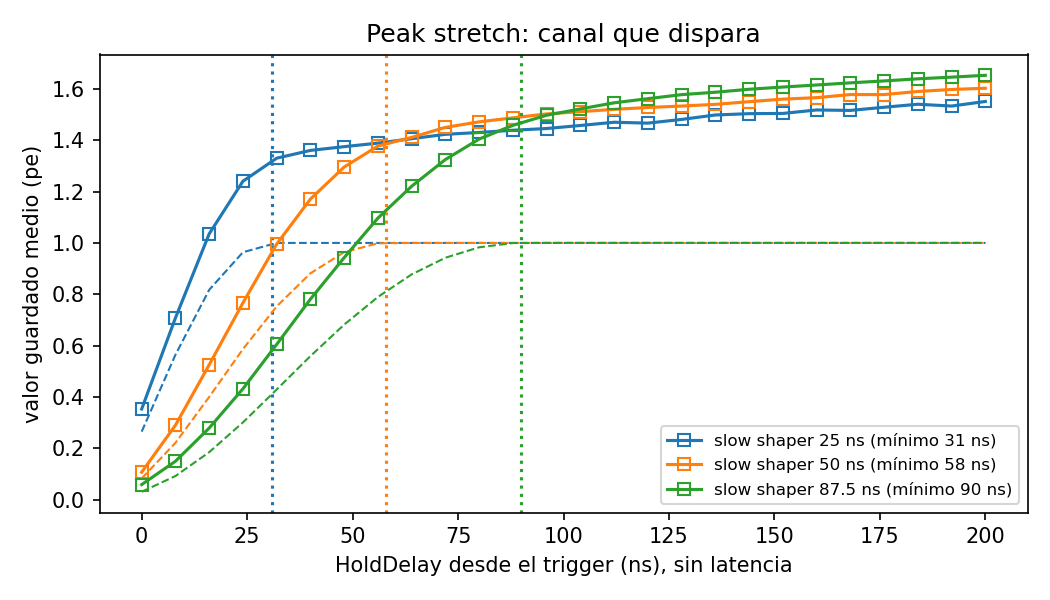
\includegraphics[width=0.65\textwidth]{scan_ps.png}
\caption{Valor medio guardado en el canal que dispara, frente al
\texttt{HoldDelay}, a 25, 50 y 87,5~ns de shaping, sin latencia. A trazos,
una avalancha sola sin ruido; los cuadrados, un modelo sencillo con ruido,
DP a 4,4~MHz y crosstalk del 19,5\,\% (5~V), de ahí que pase de 1~pe. Las
líneas de puntos marcan el \texttt{HoldDelay} mínimo según el modelo: 31, 58
y 90~ns. En los datos las curvas se desplazan a la izquierda en la latencia
de la tarjeta, que retrasa el comienzo de la ventana. La media crece
también después del codo, por el crosstalk y los DP que caen en la ventana;
el codo se lee mejor en la posición del pico de 1~pe (Sección~\ref{sec:datos}).}
\label{fig:scan}
\end{figure}

\begin{itemize}
\item Con los SiPM por encima de la tensión de ruptura (breakdown voltage,
  BV), cada canal da pulsos oscuros (dark pulses, DP), varios MHz por canal.
  Casi todos son de un fotoelectrón (pe); algunos encienden otras celdas por
  crosstalk y son de 2 o 3~pe.
\item Cuando un DP cruza el umbral del discriminador, el canal dispara. La
  tarjeta abre la ventana con un retraso propio que no conocemos (la
  latencia) y manda el hold \texttt{HoldDelay} después. En peak stretch el
  chip guarda el máximo de la salida del slow shaper (SS) dentro de esa
  ventana.
\item Si el hold llega antes del máximo del pulso, el valor guardado se queda
  en la subida y es menor que 1~pe. Si llega después, el valor guardado es el
  máximo. El valor medio guardado crece con el \texttt{HoldDelay} y se
  estabiliza cuando la ventana contiene el máximo
  (Figura~\ref{fig:scan}). El codo de esa curva es el \texttt{HoldDelay}
  mínimo: por debajo se pierde señal. Como la ventana empieza con la
  latencia, el codo llega antes que en el modelo, en la latencia.
\item Si la latencia es mayor que el tiempo entre el cruce y el máximo del
  pulso, la ventana empieza después del máximo: la curva no tiene subida, y
  su meseta queda por debajo del máximo. Según el modelo, eso pasaría con
  25~ns de shaping si la latencia pasa de 31~ns; con 50 y 87,5~ns el máximo
  llega más tarde (58 y 90~ns).
\item Más allá del codo el valor medio sigue subiendo despacio: la ventana
  más larga recoge más a menudo otro DP mayor que el que disparó.
\end{itemize}



\subsection*{Un solo canal dispara}

\begin{itemize}
\item El hold es común a los 64 canales. Si dispara cualquiera de ellos
  (el OR de los 64), cada canal es el que dispara solo en uno de cada 64
  eventos; en los demás su ventana cae en un instante cualquiera respecto a
  sus propios DP.
\item El scan del DAQ guarda, para cada canal y cada \texttt{HoldDelay}, el
  espectro de alta ganancia, sin saber qué canal disparó. Para que el
  espectro de un canal sea el del canal que dispara, el trigger se limita a
  ese canal con la máscara de la lógica de trigger
  (\texttt{Tlogic\_Mask0}, \texttt{Tlogic\_Mask1}). El DAQ no anota en
  cada evento qué canal disparó: lo sabemos porque, con la máscara, solo
  ese canal puede disparar. Los demás pueden cruzar su umbral, pero no
  generan trigger.
\item Mirar pocos canales sesga poco la medida. La latencia es de la FPGA y
  la misma para los 64 canales; el tiempo hasta el máximo lo fija el
  shaping, común a los 32 canales de cada chip; y la forma del pulso es la
  de un mismo modelo de SiPM. De un canal a otro cambian unos pocos ns (el
  umbral efectivo de cada discriminador y la dispersión de los componentes),
  menos que el paso de 8~ns del scan. El riesgo es elegir un canal raro (un
  SiPM ruidoso, un umbral desplazado): por eso se miran dos canales en cada
  chip, y en la staircase el canal elegido debe parecerse a los demás.
\item Los otros 63 canales siguen grabándose: dan, de propina, el valor
  guardado en una ventana cualquiera frente a su longitud, el pedestal y la
  escalera de 0, 1, 2~pe por encima del BV, que se compara con la
  simulación.
\end{itemize}

\subsection*{El umbral: staircase}
\label{sec:umbral}

\begin{figure}[htbp!]
\centering
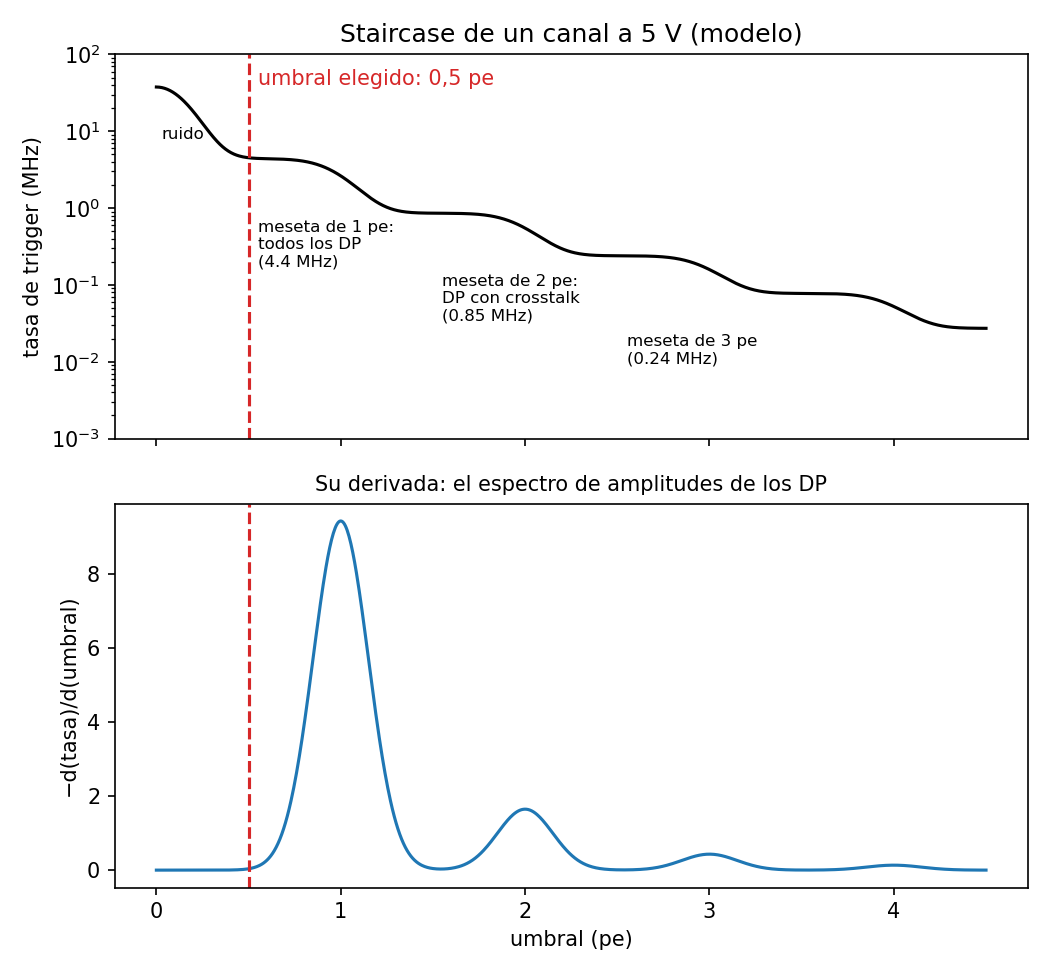
\includegraphics[width=0.7\textwidth]{staircase.png}
\caption{Staircase de un canal a 5~V según el modelo: DP a 4,4~MHz,
crosstalk del 19,5\,\% y ruido de 0,15~pe en el fast shaper. Arriba, tasa de
trigger frente al umbral, en pe; en los datos el eje es el valor de
\texttt{TD\_CoarseThreshold}. Abajo, su derivada, el espectro de amplitudes
de los DP. La línea roja marca el umbral elegido.}
\label{fig:staircase}
\end{figure}

\begin{itemize}
\item El canal tiene que dispararse con 0,5~pe, pero el umbral no está en
  pe: \texttt{TD\_CoarseThreshold} es un valor de DAC, común a los canales
  de la tarjeta, y lo que vale en pe depende de \texttt{HG\_Gain}, del
  overvoltage (la tensión por encima del BV) y de la forma del pulso. Se
  fija con la staircase.
\item {\bf Qué hace:} el DAQ recorre \texttt{TD\_CoarseThreshold} de mayor a
  menor y mide la tasa de trigger de cada canal.
\item {\bf Qué se obtiene} (Figura~\ref{fig:staircase}, arriba): a oscuras,
  la tasa baja en escalones. Con el umbral dentro del ruido la tasa es
  enorme. Entre el ruido y 1~pe la tasa es casi constante, la meseta de
  1~pe: dispara cualquier DP, unos 4,4~MHz por canal a 5~V según el modelo.
  Por encima de 1~pe solo disparan los DP con crosstalk: la meseta de 2~pe,
  unas cinco veces más baja. Y así sucesivamente. La derivada de la curva
  (abajo) es el espectro de amplitudes de los DP.
\item {\bf Qué valor buscamos:} el escalón de 1 a 2~pe está en 1~pe y el de
  2 a 3~pe en 2~pe; su distancia es 1~pe en unidades de DAC. El umbral se
  pone media distancia por debajo del escalón de 1 a 2~pe: eso es 0,5~pe, al
  principio de la meseta de 1~pe, justo fuera del ruido. Si los canales no
  coinciden, se toma el valor que deja a todos dentro de su meseta.
\item {\bf De propina:} la altura de las mesetas da la tasa de DP y el
  crosstalk, que se comparan con el modelo.
\end{itemize}

\section*{Programa de festejos}

\noindent {\bf Setup}
\begin{itemize}
\item {\bf Acción:}
  \begin{itemize}
  \item Montar sin cristal, con los SiPM conectados y a oscuras.
  \item Partir de la configuración de producción y cambiar en la pestaña
    {\bf Acquisition} solo los parámetros de la Sección~\ref{sec:janus}.
  \item \texttt{HV\_Vbias} para 5~V de overvoltage: unos 43~V a temperatura
    ambiente. Fijarlo antes de lanzar nada.
  \item Lanzar un run corto (nota 0) para que la tarjeta reciba la
    configuración y la tensión.
  \item En la pestaña {\bf Hardware}, encender el HV de la tarjeta y esperar
    a que Vmon e Imon estén estables.
  \end{itemize}
\item {\bf Precaución:} el DAQ todavía no aplica \texttt{FastShaperInput}
  (es uno de los cambios que JMB está revisando). La staircase del paso~1
  deja el fast shaper en la alta ganancia, que es lo que queremos. Hacer
  siempre la staircase primero y no apagar la tarjeta entre la staircase y
  los scans.
\end{itemize}

\noindent {\bf Paso 1: staircase}
\begin{itemize}
\item {\bf Acción:}
  \begin{itemize}
  \item En la pestaña {\bf Scans}, Staircase: \texttt{Minimum} = 150,
    \texttt{Maximum} = 300, \texttt{Step} = 1, \texttt{Dwell} = 500~ms. Si
    las mesetas no caen en ese rango, repetir con \texttt{Minimum} = 0,
    \texttt{Maximum} = 600, \texttt{Step} = 2.
  \item {\bf Start scan}.
  \end{itemize}
\item {\bf Resultado:} la tasa de trigger de cada canal frente al umbral, en
  la gráfica de la pestaña y guardada como un run con su número.
\item {\bf Acción:}
  \begin{itemize}
  \item Elegir en las curvas el valor de 0,5~pe (Sección~\ref{sec:umbral}).
  \item Ponerlo en \texttt{TD\_CoarseThreshold}.
  \end{itemize}
\end{itemize}

\noindent {\bf Paso 2: scan con slow shaper de 25~ns}
\begin{itemize}
\item {\bf Acción:}
  \begin{itemize}
  \item \texttt{HG\_ShapingTime} = 25~ns.
  \item Trigger solo del canal~0: \texttt{Tlogic\_Mask0} = 0x00000001,
    \texttt{Tlogic\_Mask1} = 0x00000000.
  \item Un run corto (nota 0), para que la tarjeta reciba el umbral, el
    shaping y la máscara.
  \item En la pestaña {\bf Scans}, Hold-delay scan: \texttt{Minimum} = 0~ns,
    \texttt{Maximum} = 248~ns, \texttt{Step} = 8~ns, \texttt{Events / delay}
    = 10\,000, \texttt{Timeout} = 30~s.
  \item {\bf Start scan}.
  \end{itemize}
\item {\bf Resultado:} 32 puntos; para cada canal, el espectro de alta
  ganancia frente al \texttt{HoldDelay}, en el mapa de la pestaña y
  guardado como un run con su número.
\end{itemize}

\noindent {\bf Paso 3: scan con slow shaper de 50~ns}
\begin{itemize}
\item {\bf Acción:} como el paso~2 (con su run corto), con
  \texttt{HG\_ShapingTime} = 50~ns y \texttt{Maximum} = 496~ns,
  \texttt{Step} = 16~ns.
\item {\bf Resultado:} 32 puntos, guardados como un run.
\end{itemize}

\noindent {\bf Paso 4: scan con slow shaper de 87,5~ns}
\begin{itemize}
\item {\bf Acción:} como el paso~3 (con su run corto), con
  \texttt{HG\_ShapingTime} = 87,5~ns.
\item {\bf Resultado:} 32 puntos, guardados como un run.
\end{itemize}

\noindent {\bf Paso 5: otros canales}
\begin{itemize}
\item {\bf Acción:} como el paso~2 (25~ns), un scan por canal, cambiando
  solo la máscara y con un run corto antes de cada scan (los canales 0 a 31 están en el primer chip y los 32 a 63
  en el segundo):
  \begin{itemize}
  \item Canal~20 (primer chip): \texttt{Tlogic\_Mask0} = 0x00100000,
    \texttt{Tlogic\_Mask1} = 0x00000000.
  \item Canal~40 (segundo chip): \texttt{Tlogic\_Mask0} = 0x00000000,
    \texttt{Tlogic\_Mask1} = 0x00000100.
  \item Canal~60 (segundo chip): \texttt{Tlogic\_Mask0} = 0x00000000,
    \texttt{Tlogic\_Mask1} = 0x10000000.
  \end{itemize}
\item {\bf Resultado:} 3 scans de 32 puntos, cada uno guardado como un run.
\item {\bf Análisis:} los codos deben coincidir con el del paso~2 dentro de
  un paso de 8~ns; si los dos canales de un chip coinciden entre sí pero no
  con los del otro, la latencia o el shaping son distintos en los dos chips.
\end{itemize}

\noindent {\bf Al terminar}
\begin{itemize}
\item {\bf Acción:} devolver \texttt{Tlogic\_Mask0} y \texttt{Tlogic\_Mask1}
  a 0xFFFFFFFF y \texttt{BunchTrgSource} y \texttt{TriggerLogic} a sus
  valores de partida.
\end{itemize}

\section*{Qué necesita el cocinero}

\begin{itemize}
\item La staircase y los seis scans: en la pestaña {\bf Runs}, cada uno
  con su número y su fichero.
\item Una fila por staircase y por scan en el logbook de la hoja de Google
  (nota 0), con el shaping, el canal que dispara y el umbral.
\item Si algo no se comporta como espera el menú, para y grita.
\end{itemize}

\section{Cómo entra la medida en el modelo}
\label{sec:razon}

\begin{itemize}
\item El modelo pasa una avalancha de 1~pe sin ruido por el preamplificador,
  el fast shaper y el slow shaper del Citiroc (menú~1, Figura~1): el fast
  shaper da el instante del trigger y el slow shaper el de su máximo. La
  diferencia es el \texttt{HoldDelay} mínimo sin latencia: 31~ns a 25~ns,
  58~ns a 50~ns y 90~ns a 87,5~ns.
\item El codo del modelo menos el medido da la latencia de la tarjeta, que
  dice qué parte del pulso cae dentro de la ventana y con qué
  \texttt{HoldDelay} usar en las medidas que disparan con la señal (la
  calibración del menú~3 usa trigger periódico y no depende de la
  latencia). Que el desplazamiento sea el mismo en los tres shapings
  comprueba la forma del pulso del modelo.
\item {\bf La regla del margen.} El \texttt{HoldDelay} de las medidas que
  disparan con la señal (las de energía) se pone uno o dos pasos (8 a 16~ns) por encima del codo, por dos
  razones. El codo varía unos ns de un canal a otro, y el
  \texttt{HoldDelay} es común a los 64. Y un DP de 2 o 3~pe cruza el umbral
  antes que uno de 1~pe, mientras que su máximo llega a la misma hora: del
  trigger al máximo pasa más tiempo, y el codo de esos pulsos llega unos ns
  más tarde. En peak stretch, pasarse un poco solo cuesta una ventana algo
  más larga (el pedestal sube un poco, menú~1); quedarse corto pierde señal.
\item El valor de la meseta, en cuentas de ADC, es una primera estimación de
  la ganancia (la buena sale del menú~3) y dice si los picos de 1~pe se
  separan del pedestal con el \texttt{HG\_Gain} elegido.
\item Los 63 canales que no disparan dan el valor guardado en una ventana
  cualquiera frente a su longitud, con DP: la simulación lo reproduce con el
  mismo peak stretch.
\end{itemize}

\section{Parámetros del DAQ (A5202)}
\label{sec:janus}

\begin{center}
\small
\begin{tabular}{p{0.3\textwidth} p{0.6\textwidth}}
\hline
parámetro & valor \\
\hline
\texttt{HV\_Vbias} & 5~V por encima del BV: unos 43~V a temperatura
ambiente \\
\texttt{HV\_IndivAdj} & 0 (como en producción) \\
\texttt{AcquisitionMode} & SPECTROSCOPY \\
\texttt{BunchTrgSource} & TLOGIC (la lógica de trigger) \\
\texttt{TriggerLogic} & OR64 \\
\texttt{Tlogic\_Mask0}, \texttt{Tlogic\_Mask1} & solo el canal que dispara
(pasos 2 a 5) \\
\texttt{TD\_CoarseThreshold} & el de 0,5~pe (paso 1) \\
\texttt{FastShaperInput} & HG-PA (ver la precaución del Setup) \\
\texttt{HG\_ShapingTime} & 25, 50 o 87,5~ns, según el paso \\
\texttt{LG\_ShapingTime} & 87,5~ns \\
\texttt{HG\_Gain}, \texttt{LG\_Gain} & 55 (como en producción) \\
\texttt{GainSelect} & BOTH \\
\texttt{ZS\_Threshold\_HG}, \texttt{ZS\_Threshold\_LG} & 0, también en los
umbrales por canal si la configuración los tiene \\
\texttt{ChEnableMask0}, \texttt{ChEnableMask1} & todos los canales
({\bf Configure channels}, {\bf Enable all}) \\
\hline
\end{tabular}
\end{center}

\noindent Los parámetros con índice del fichero de producción (por ejemplo
\texttt{TD\_CoarseThreshold[0]} o \texttt{ChEnableMask0[1]}) son de cada
tarjeta y mandan sobre el valor común: cambiarlos también, o quitarlos
(nota 0).

\section{Análisis}
\label{sec:datos}

\begin{itemize}
\item {\bf Staircase:} para cada canal, la tasa frente al umbral; el valor
  de 0,5~pe, la altura de las mesetas de 1 y 2~pe (la tasa de DP) y su
  cociente (el crosstalk).
\item {\bf Scans:} para el canal que dispara y cada \texttt{HoldDelay}, la
  media del espectro de alta ganancia menos el pedestal, y la posición del
  pico de 1~pe. El codo es el \texttt{HoldDelay} a partir del cual la
  posición del pico deja de crecer. Los espectros del scan tienen 512
  canales de 16 cuentas de ADC: bastan para la posición del pico, no para
  su anchura.
\item {\bf Los otros canales:} la fracción de eventos por encima de 0,5~pe
  frente al \texttt{HoldDelay}.
\end{itemize}

\section{Lo que se espera, según el modelo}

\begin{itemize}
\item {\bf Staircase:} la meseta de 1~pe a unos 4,4~MHz por canal y la de
  2~pe unas cinco veces más baja.
\item {\bf Scans:} la curva de la Figura~\ref{fig:scan}, con el codo a 31,
  58 y 90~ns menos la latencia. Si con 25~ns la curva es plana desde
  \texttt{HoldDelay} = 0, la latencia es mayor que 31~ns.
\item {\bf Los otros canales:} la fracción por encima de 0,5~pe crece con
  la ventana, del orden de la tasa de DP por la longitud de la ventana.
\end{itemize}

\end{document}
